%%%% Better Poster latex template example v1.0 (2019/04/04)
%%%% GNU General Public License v3.0
%%%% Rafael Bailo
%%%% https://github.com/rafaelbailo/betterposter-latex-template
%%%%
%%%% Original design from Mike Morrison
%%%% https://twitter.com/mikemorrison

\documentclass[a0paper,fleqn]{betterposter}

\usepackage[latin1]{inputenc}
\usepackage{tikz}
\usetikzlibrary{shapes,arrows}


% Define block styles
\tikzstyle{decision} = [diamond, draw, fill=blue!20,
    text width=4.5em, text badly centered, node distance=10em, inner sep=0pt]
\tikzstyle{block} = [rectangle, draw, fill=blue!20,
    text width=6em, text centered, rounded corners, minimum height=4em, node distance = 10em]
\tikzstyle{line} = [draw, -latex', line width=.25mm]
\tikzstyle{cloud} = [draw, ellipse,fill=red!20, node distance=15em,
    minimum height=2em]

%%%% Uncomment the following commands to customise the format

%% Setting the width of columns
% Left column
%\setlength{\leftbarwidth}{0.25\paperwidth}
% Right column
%\setlength{\rightbarwidth}{0.25\paperwidth}

%% Setting the column margins
% Horizontal margin
%\setlength{\columnmarginvertical}{0.05\paperheight}
% Vertical margin
%\setlength{\columnmarginhorizontal}{0.05\paperheight}
% Horizontal margin for the main column
%\setlength{\maincolumnmarginvertical}{0.15\paperheight}
% Vertical margin for the main column
%\setlength{\maincolumnmarginhorizontal}{0.15\paperheight}

%% Changing font sizes
% Text font
%\renewcommand{\fontsizestandard}{\fontsize{28}{35} \selectfont}
% Main column font
%\renewcommand{\fontsizemain}{\fontsize{28}{35} \selectfont}
% Title font
%\renewcommand{\fontsizetitle}{\fontsize{28}{35} \selectfont}
% Author font
%\renewcommand{\fontsizeauthor}{\fontsize{28}{35} \selectfont}
% Section font
%\renewcommand{\fontsizesection}{\fontsize{28}{35} \selectfont}

%% Changing font sizes for a specific text segment
% Place the text inside brackets:
% {\fontsize{28}{35} \selectfont Your text goes here}

%% Changing colours
% Background of side columns
%\renewcommand{\columnbackgroundcolor}{black}
% Font of side columns
%\renewcommand{\columnfontcolor}{gray}
% Background of main column
%\renewcommand{\maincolumnbackgroundcolor}{empirical}
%\renewcommand{\maincolumnbackgroundcolor}{theory}
%\renewcommand{\maincolumnbackgroundcolor}{methods}
%\renewcommand{\maincolumnbackgroundcolor}{intervention}
% Font of main column
%\renewcommand{\maincolumnfontcolor}{gray}

\begin{document}
\betterposter{
%%%%%%%% MAIN COLUMN

\maincolumn{
%%%% Main space

\textbf{Function-Fiasco} is an automatic tool that detects pseudo-tested methods in Python progams.
}{
%%%% Bottom space

%% QR code
\qrcode{img/qrcode}{img/smartphoneWhite}{
\textbf{Take a picture} to
\\download the full paper
}
% Smartphone icon
% Author: Freepik
% Retrieved from: https://www.flaticon.com/free-icon/smartphone_65680

%% Compact QR code (comment the previous command and uncomment this one to switch)
%\compactqrcode{img/qrcode}{
%\textbf{Take a picture} to
%\\download the full paper
%}

}

}{
%%%%%%%% LEFT COLUMN

\title{The Title}
\author{Nicholas Tocci}
\author{Gregory Kapfhammer}

\section{Introduction}
Software systems are very large and complex. Because of this, modern python
programs are difficult to test due to the lack of type safety. Another concern is
the possible misleading nature of statement coverage since it doesn't factor in
branches and iteration, there is no information on the data state, and the quality
of the oracle. Due to this, there is a potential chance for psuedo-tested methods
to exist in python programs.

\begin{center}
% Linear regression
% Author: Henri Menke
% Retrieved from: http://www.texample.net/tikz/examples/linear-regression/

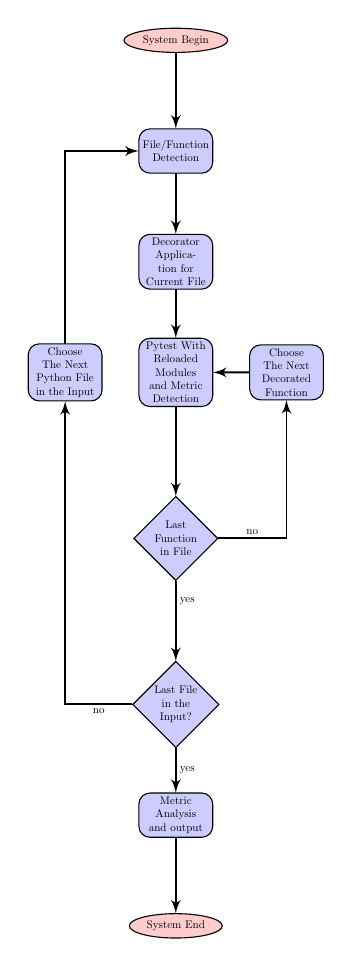
\begin{tikzpicture}[auto, scale=5, every node/.style={scale=0.4}]
    \node [cloud] (sys) {System Begin};
    \node [block, below of=sys, node distance=10em] (file) {File/Function Detection};
    \node [block, below of=file, node distance=10em] (Decorator) {Decorator Application for Current File};
    \node [block, below of=Decorator] (pytest) {Pytest With Reloaded Modules and Metric Detection};
    \node [block, right of=pytest, node distance=10em] (choose) {Choose The Next Decorated Function};
    \node [block, left of=pytest] (Next) {Choose The Next Python File in the Input};
    \node [decision, below of=pytest, node distance=15em] (function) {Last Function in File};
    \node [decision, below of=function, node distance=15em] (Last) {Last File in the Input?};
    \node [block, below of=Last, node distance=10em] (Metric) {Metric Analysis and output};
    \node [cloud, below of=Metric, node distance=10em] (end) {System End};


    \path [line] (sys) -- (file);
    \path [line] (file) -- (Decorator);
    \path [line] (Decorator) -- (pytest);
    \path [line] (pytest) -- (function);
    \path [line] (choose) -- (pytest);
    \path [line] (function) -| node [near start] {no} (choose);
    \path [line] (function) -- node [near start] {yes} (Last);
    \path [line] (Last) -| node [near start] {no} (Next);
    \path [line] (Next) |- (file);
    \path [line] (Last) -- node {yes} (Metric);
    \path [line] (Metric) -- (end);

\end{tikzpicture}

\end{center}


%% Institution logo

\includegraphics[width=\textwidth]{img/logo}\\

}{
%%%%%%%% RIGHT COLUMN

Here you can add \textbf{supplementary material}. For instance, a new diagram:
\begin{center}
% Commutative diagram with edges passing under/over
% Author: Stefan Kottwitz, http://texblog.net/
% Retrieved from: http://www.texample.net/tikz/examples/commutative-diagram/
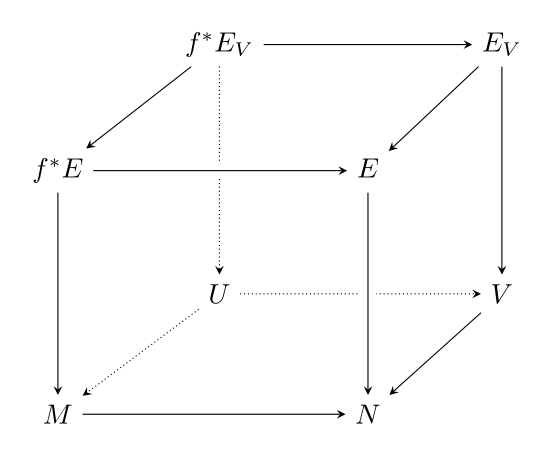
\includegraphics[width=\textwidth]{img/tikzexample2}
\end{center}

Some cute ducklings:
\begin{center}
% Picture of ducklings
% Author: Magda Ehlers, https://www.pexels.com/@magda-ehlers-pexels
% Retrieved from: https://www.pexels.com/photo/selective-focus-photo-of-flock-of-ducklings-perching-on-gray-concrete-pavement-1300355/
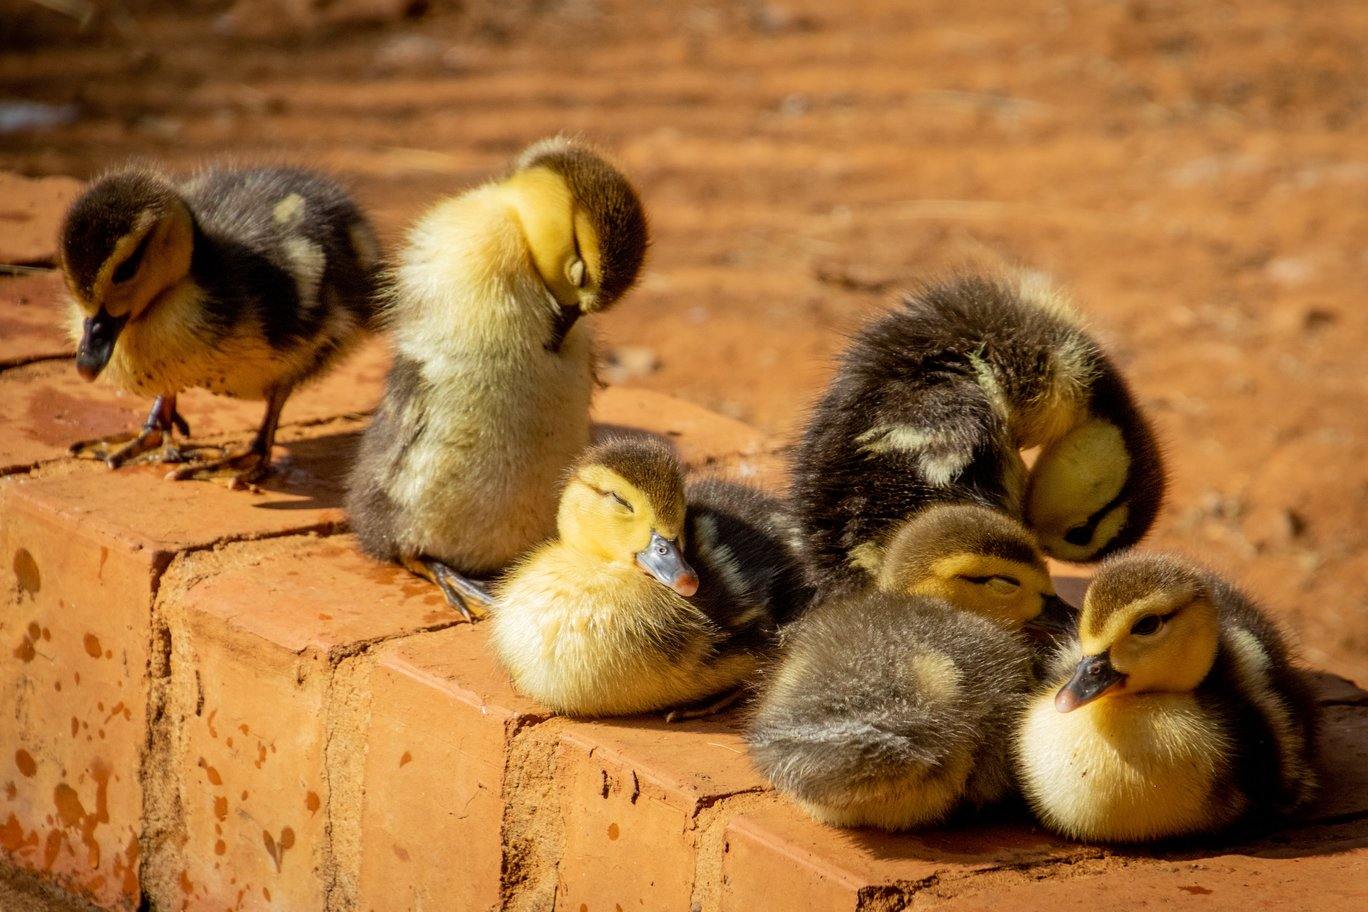
\includegraphics[width=\textwidth]{img/ducklings}
\end{center}
}
\end{document}
